%%mark = star, diamond, square, otimes
%\documentclass{article}
%\usepackage{pgfplots}
%\usepackage[justification=centering]{caption}
%\pgfplotsset{compat=newest}
%\begin{document}
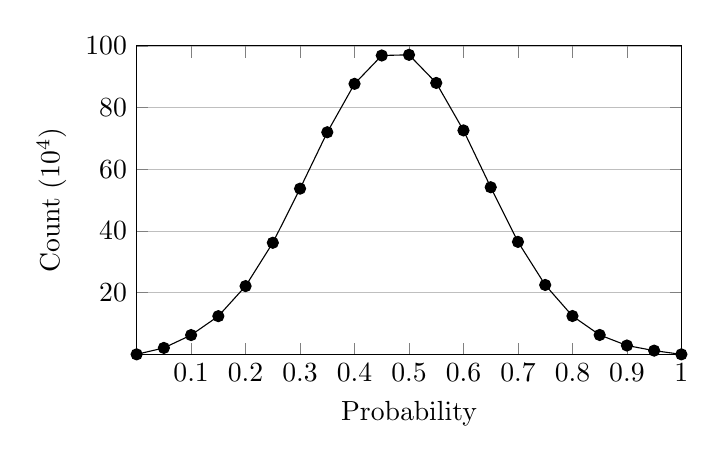
\begin{tikzpicture}
\begin{axis}[
	width=8.5cm,
	height=5.5cm,
    xlabel={Probability },
    ylabel={Count ($10^4$)},
    xmin=0, xmax=1.0,
    ymin=0, ymax=100,
    xtick={.1,.2,.3,.4,.5,.6,.7,.8,.9,1.0},
    ytick={20,40,60,80,100},
    legend pos=north east,
    ymajorgrids=true,
    grid style={line width=.2pt,draw=gray!50},
]
 
\addplot[
    solid, every mark/.append style={solid, fill=black}, mark=*
    ]
    coordinates {
		(0			,0	)
		(.05		,2.0856	)
		(0.1 		,6.2495	)
		(0.15		,12.3806	)
		(0.2 		,22.1236	)
		(0.25		,36.1638	)
		(0.3 		,53.7087	)
		(0.35		,71.9860	)
		(0.4 		,87.6780	)
		(0.45		,96.8615	)
		(0.5 		,97.0789	)
		(0.55		,87.9683	)
		(0.6 		,72.5833	)
		(0.65		,54.1544	)
		(0.7 		,36.4540	)
		(0.75		,22.4901	)
		(0.8 		,12.4234	)
		(0.85		,6.2841	)
		(0.9 		,2.8673	)
		(0.95		,1.2048	)
		(1.0		,0	)
};
 
\end{axis}
\end{tikzpicture}
%\end{document}